\subsection*{Log ind}
Der oprettes en log ind funktion, for at skabe en individuel bruger for den enkelte KOL-patient med henblik på at sikre brugerens private oplysninger samt resultater. Aktivitetsdiagrammet over log ind fremgår af \autoref{fig:logind}. 

\begin{figure} [H]
\centering
\textbf{Aktivitetsdiagram: Log ind}\par\medskip
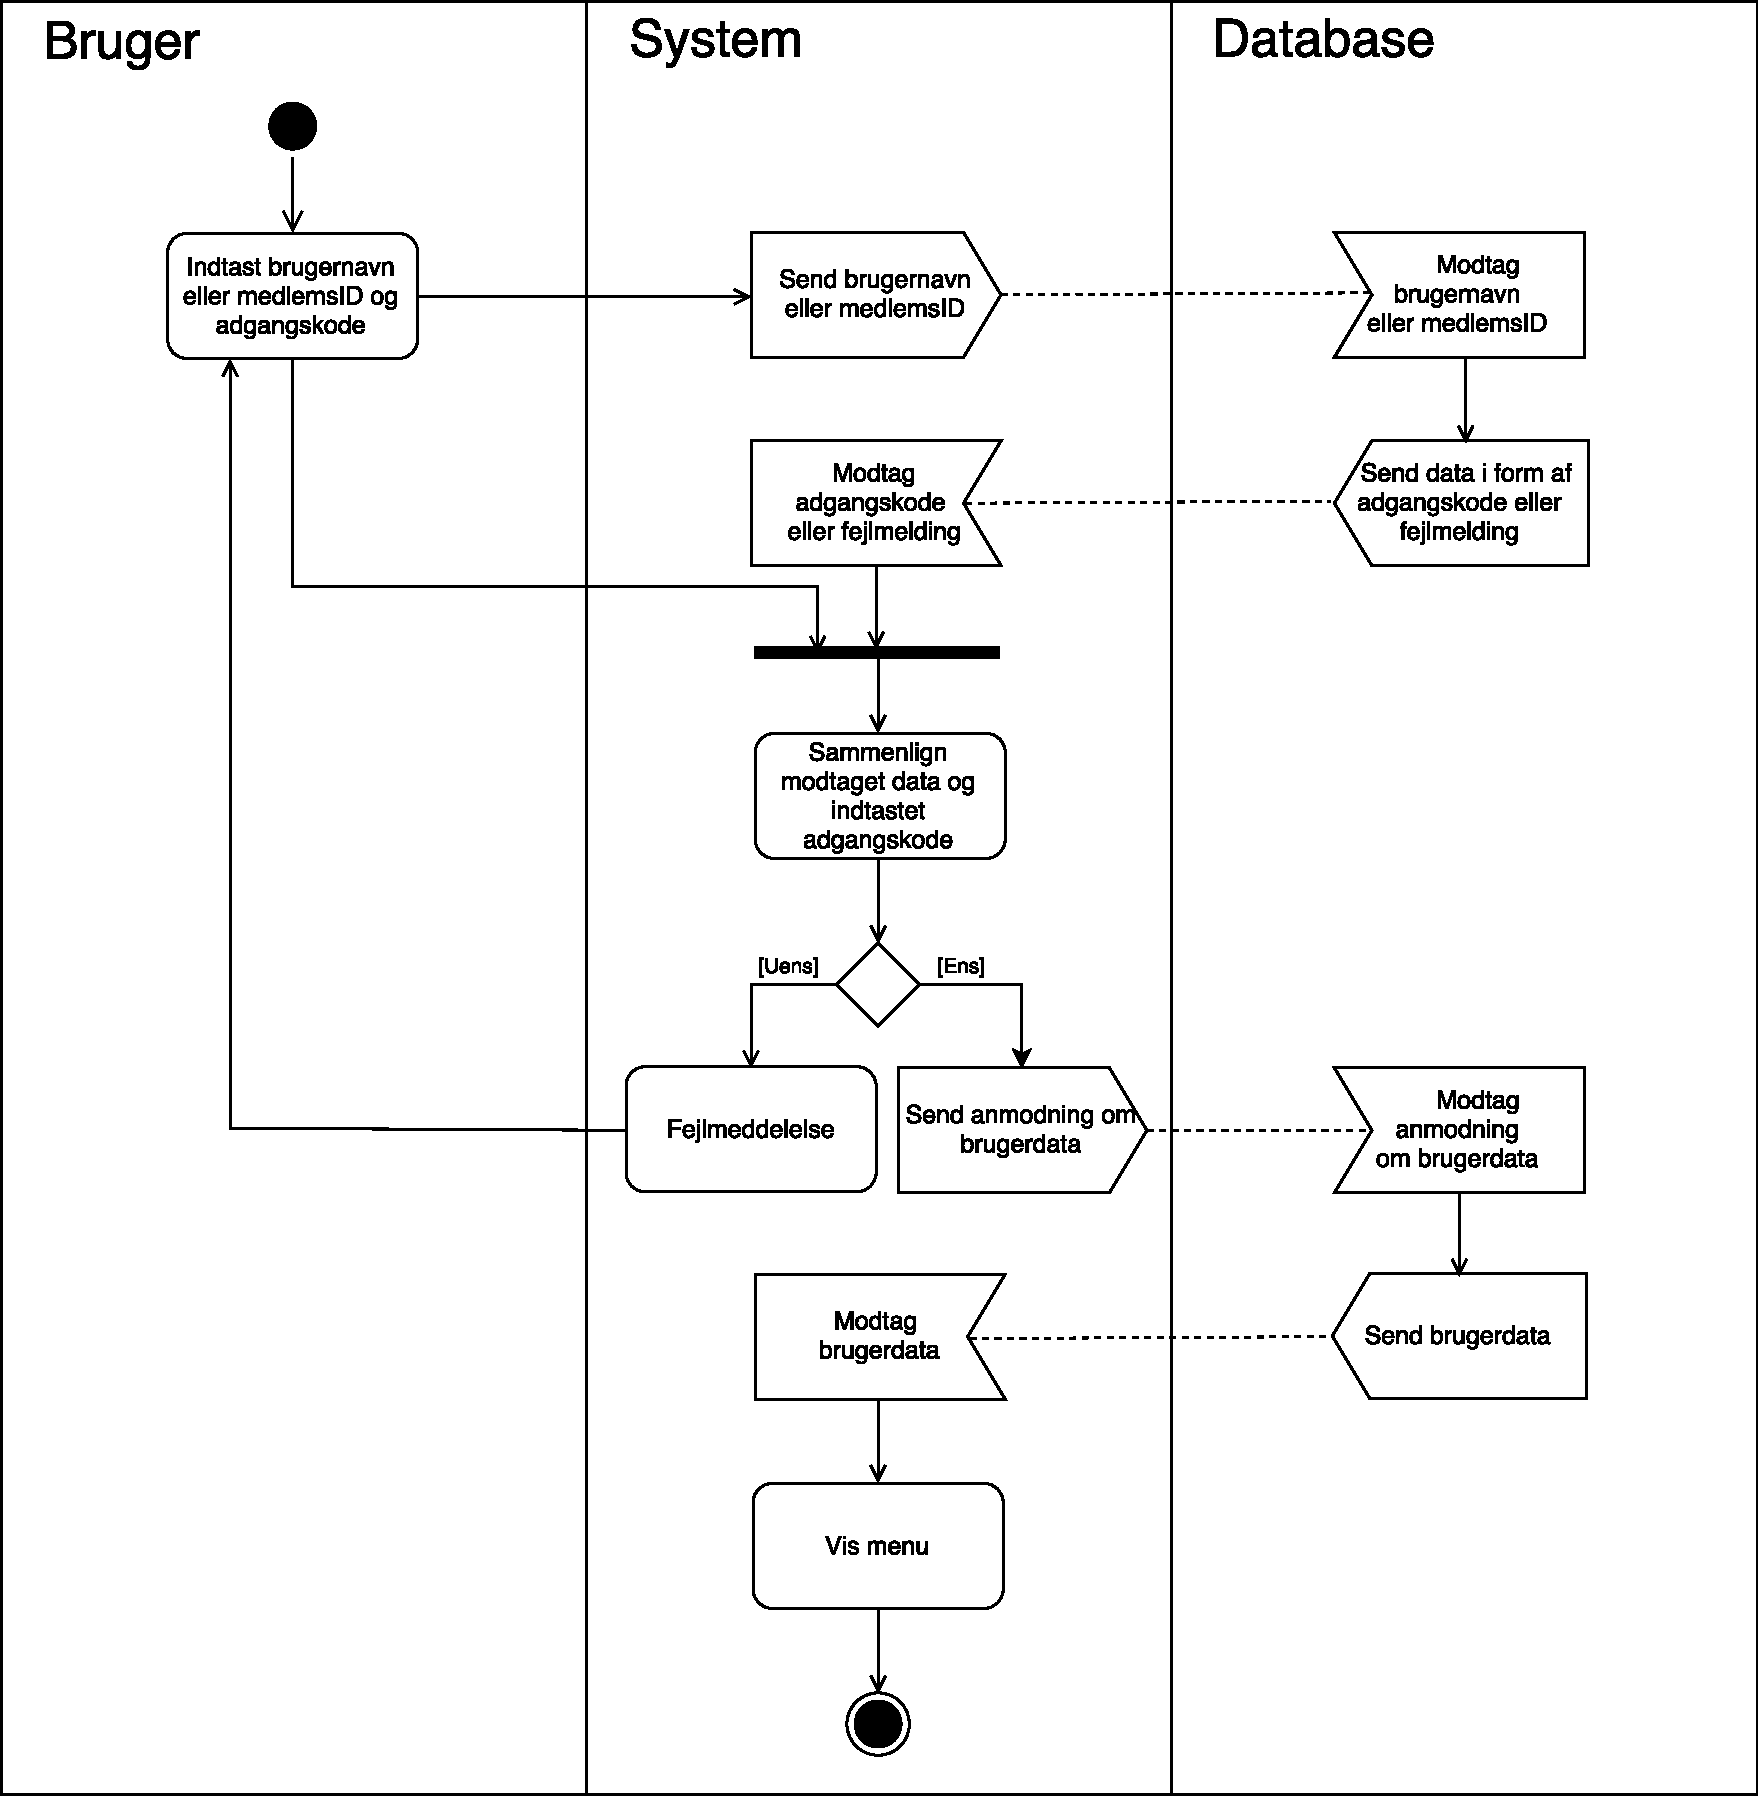
\includegraphics[width=0.9\textwidth]{figures/aktivitetsdiagram/Logind}
\caption{Aktivitetsdiagram over log ind.}
\label{fig:logind}
\end{figure}


\noindent
Når KOL-patienten vil anvende app'en skal medlemsID eller brugernavn samt kodeord indtastes. Systemet sender det indtastede medlemsID eller brugernavn til databasen, som tilbagesender det tilhørende kodeord, hvis det findes i databasen. Findes de indtastede informationer ikke, sendes en fejlmeddelelse i form af 0. Systemet sammenligner herefter brugerens indtastede adgangskode med adgangskoden fra databasen. Er de to værdier ens, har brugeren indtastet de korrekte informationer, hvortil brugerdata hentes fra databasen og hovedmenuen vises. Brugerdata omfatter brugerens informationer og tidligere resultater. Er de to værdier ikke ens, tilbagesender systemet en fejlmeddelelse, og brugeren får derefter mulighed for at indtaste log ind informationen igen. 